\section{Bipyramids}

\paragraph{Creation process: }

The whole process is very similar to the nanosheets one. The key difference is that the model becomes taller therefore more unstable. It will be necessary to lay the bipyramid down on one side. This is not a fixed rule, but statistically it's more common to find the nanoparticle on it's more stable equilibrium.

The standard model is created in Blender using a cube with a central subdivision along the Y axis. It is centered in the origin with half size equal to 1.

Several other passages are applied in order to obtain the correct model to use later, as shown in Fig. \ref{fig:bipyramids_process}:

\begin{itemize}
    \item Scale along Y axis (to match the correct ratio between height and width) equals to: $S_Y = h / w$
    \item Scale along XZ plane (to generate the insets of the superior and inferior faces) equals to: $S_{XZ} = 1 - (h_{eff} / tan(68.3^{\circ}))$
\end{itemize}

Where h\_eff is the new calculated height and $68.3^{\circ}$ is the crystalline angle of anatase $TiO_2$ from X-ray measurements.

\newpage

\begin{figure}[ht]
    \centering
    \begin{subfigure}[b]{0.3\textwidth}
        % bipi_1_1
        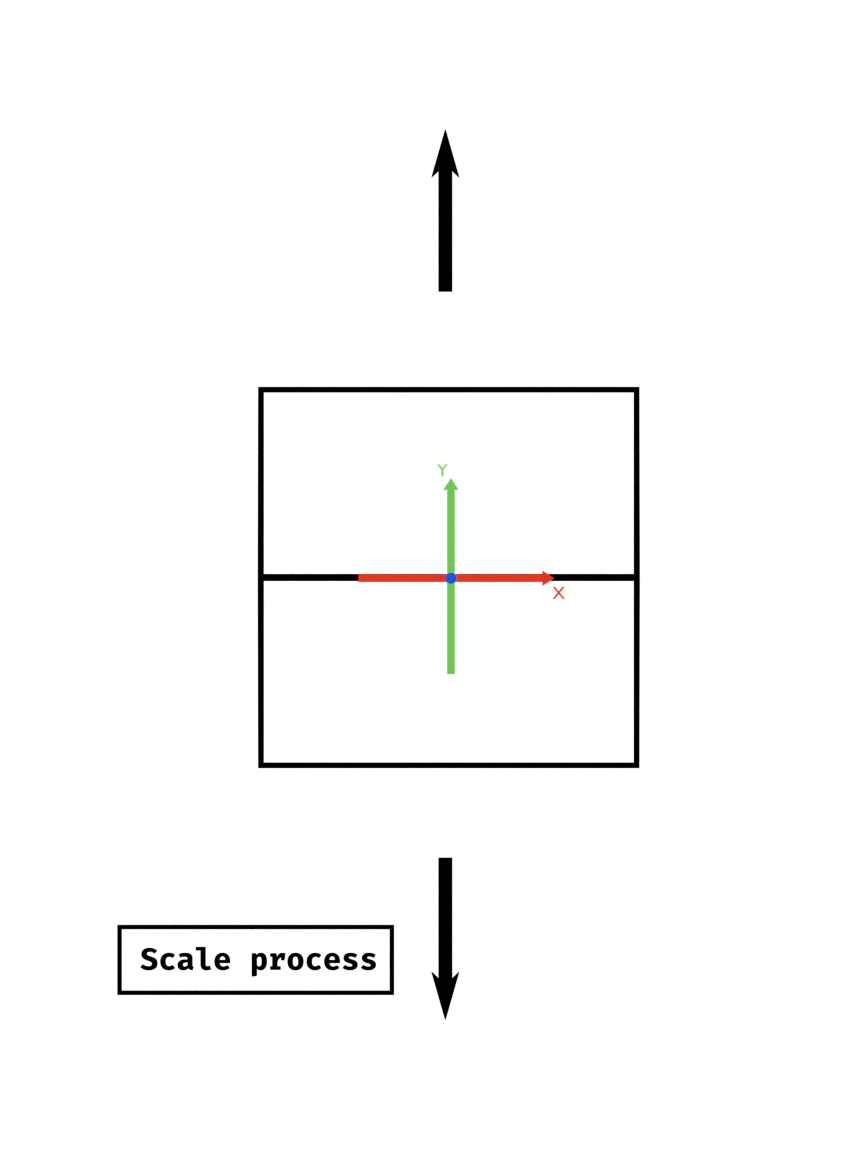
\includegraphics[width=.95\textwidth, clip]{./immagini/bipi_1_1.png}
        \caption{}
        \label{fig:bipyramids_process1}
    \end{subfigure}
    \hfill
    \begin{subfigure}[b]{0.3\textwidth}
        % bipi_1_2
        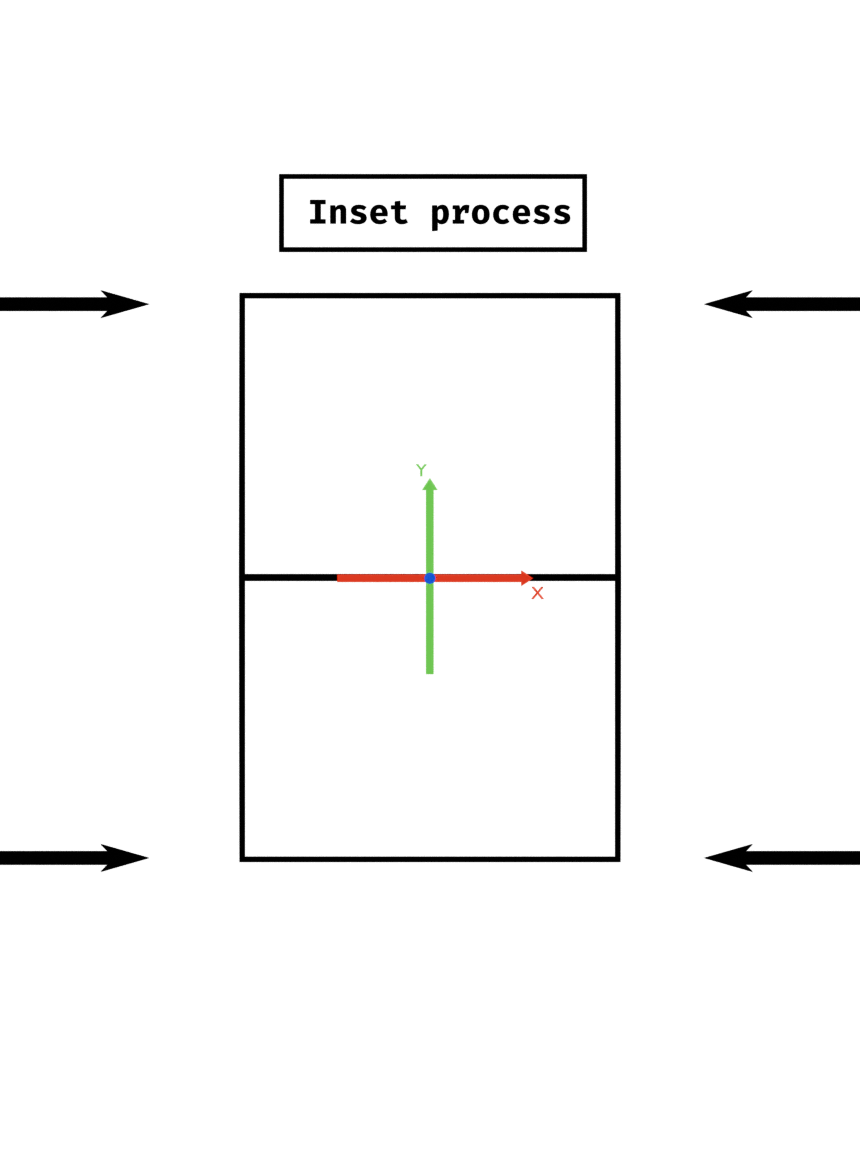
\includegraphics[width=.95\textwidth, clip]{./immagini/bipi_1_2.png}
        \caption{}
        \label{fig:bipyramids_process2}
    \end{subfigure}
    \hfill
    \begin{subfigure}[b]{0.3\textwidth}
        % bipi_1_3
        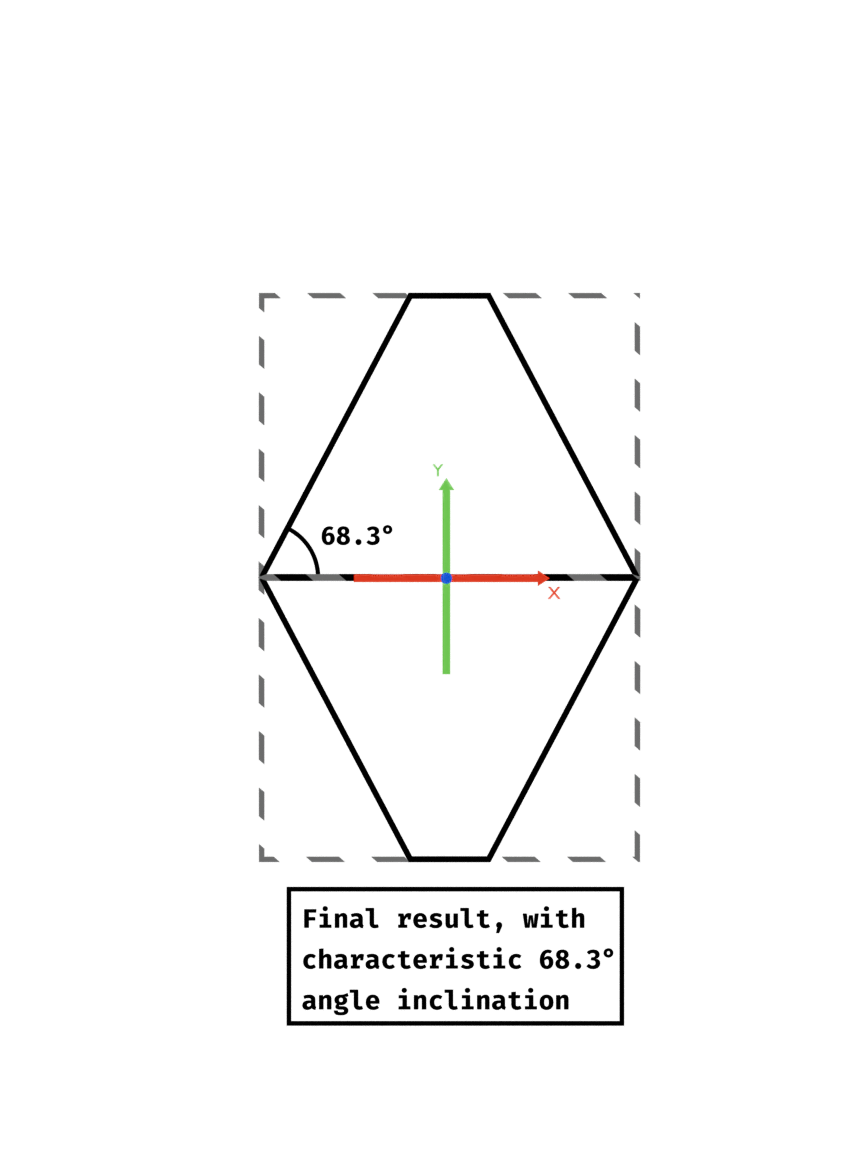
\includegraphics[width=.95\textwidth, clip]{./immagini/bipi_1_3.png}
        \caption{}
        \label{fig:bipyramids_process3}
    \end{subfigure}
    \caption{Creation steps: a) Scale along Y axis b) inset of the superior and inferior surfaces c) final standard model}
    \label{fig:bipyramids_process}
\end{figure}

\paragraph{Positioning process: }

After that, it must be positioned onto one of the diagonal faces, since the small bottom base will not ensure the maximum equilibrium. This is done by moving along the Y axis the model, so that the bottom base sits on the floor. Subsequently, a rotation matrix along the X axis is applied to rotate the bipyramid of $68.3^{\circ}$, as shown in Fig. \ref{fig:bipyramids_positioning}:

\begin{figure}[ht]
    \centering
    \begin{subfigure}[b]{0.22\textwidth}
        % bipi_2_1
        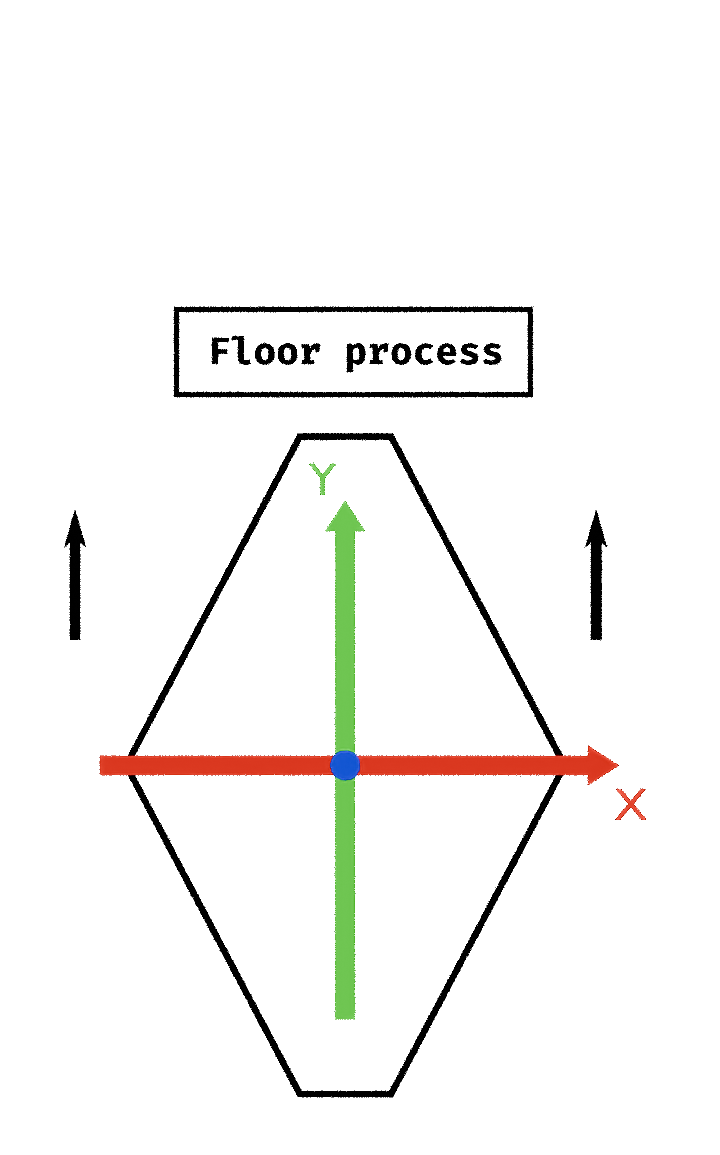
\includegraphics[width=.95\textwidth, clip]{./immagini/bipi_2_1.png}
        \caption{}
        \label{fig:bipyramids_positioning1}
    \end{subfigure}
    \hfill
    \begin{subfigure}[b]{0.22\textwidth}
        % bipi_2_2
        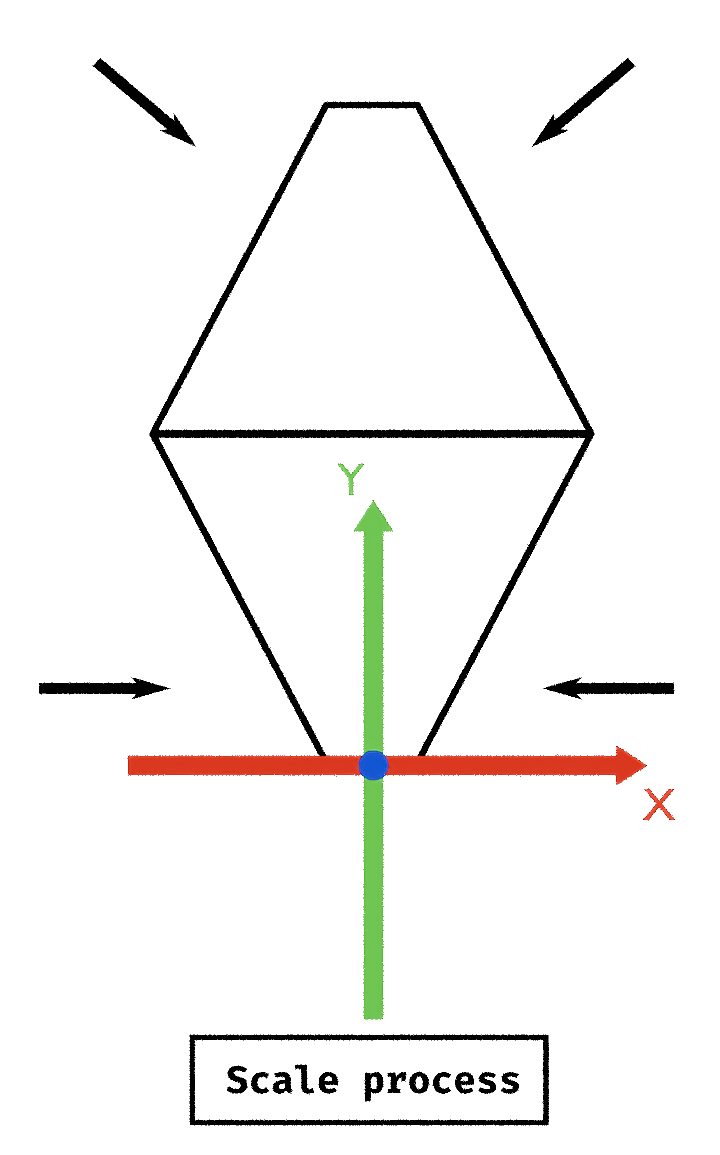
\includegraphics[width=.95\textwidth, clip]{./immagini/bipi_2_2.png}
        \caption{}
        \label{fig:bipyramids_positioning2}
    \end{subfigure}
    \hfill
    \begin{subfigure}[b]{0.22\textwidth}
        % bipi_2_3
        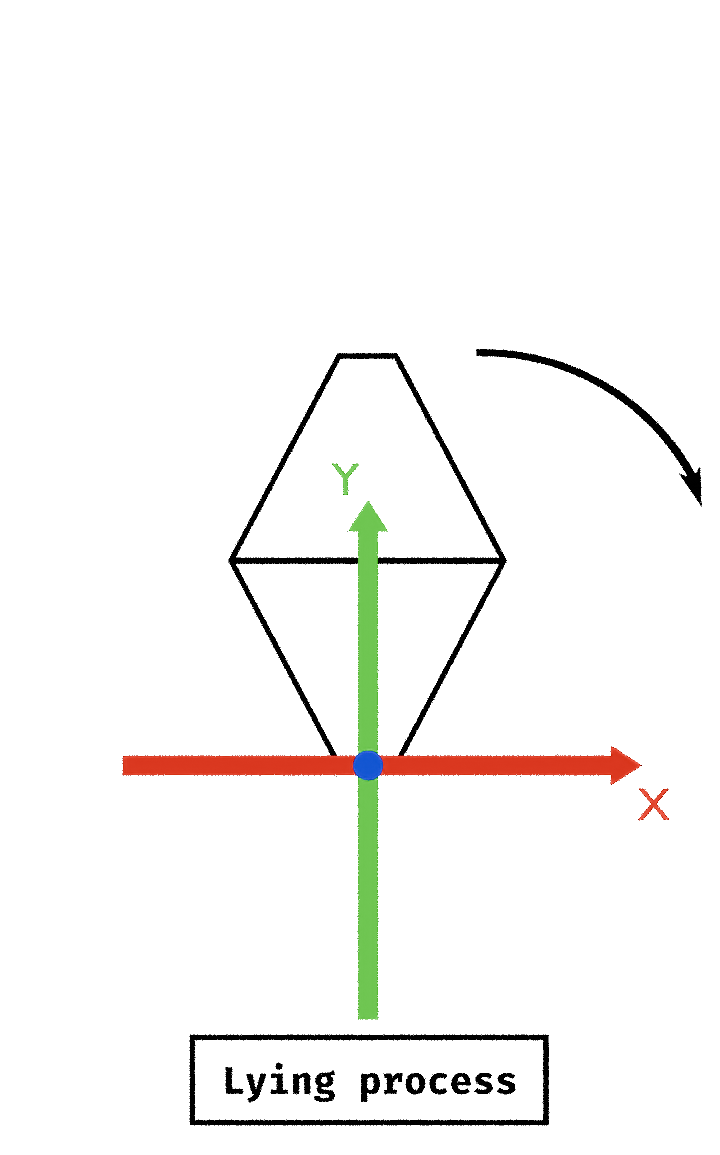
\includegraphics[width=.95\textwidth, clip]{./immagini/bipi_2_3.png}
        \caption{}
        \label{fig:bipyramids_positioning3}
    \end{subfigure}
    \hfill
    \begin{subfigure}[b]{0.22\textwidth}
        % bipi_2_4
        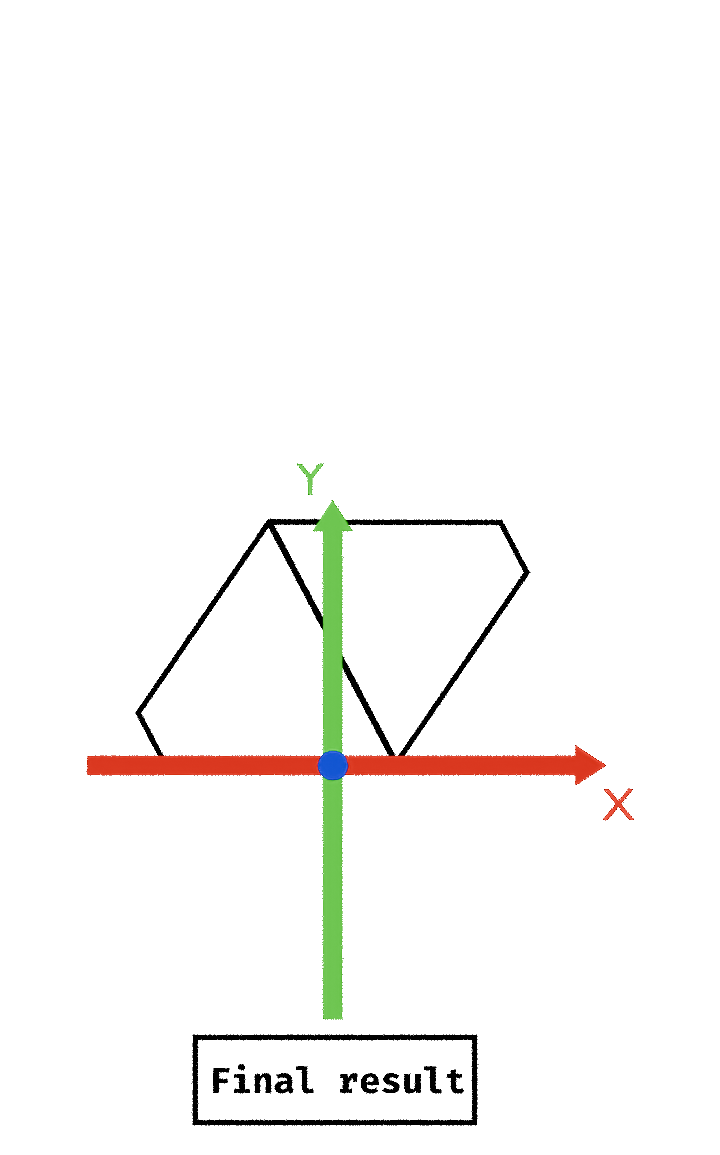
\includegraphics[width=.95\textwidth, clip]{./immagini/bipi_2_4.png}
        \caption{}
        \label{fig:bipyramids_positioning4}
    \end{subfigure}
    \caption{Instance positioning: a) floor process b) scaling process c) lying process d) final positioned model}
    \label{fig:bipyramids_positioning}
\end{figure}


\newpage

Finally, a traslation is applied in order to center the model on it's center of mass. Thus, it will be easier for the user to position and rotate the desired nanoparticles on the substrate.

\paragraph{Examples: }

Some example of generated images are reported in Fig. \ref{fig:bipiramid_type} a-c. In particular, Fig. \ref{fig:bipiramid2} and \ref{fig:bipiramid3} shown also compenetrated nanosheets that are successfully handled by this system.

\begin{figure}[ht]
    \centering
    \begin{subfigure}[b]{0.3\textwidth}
        % bipiramid_singola
        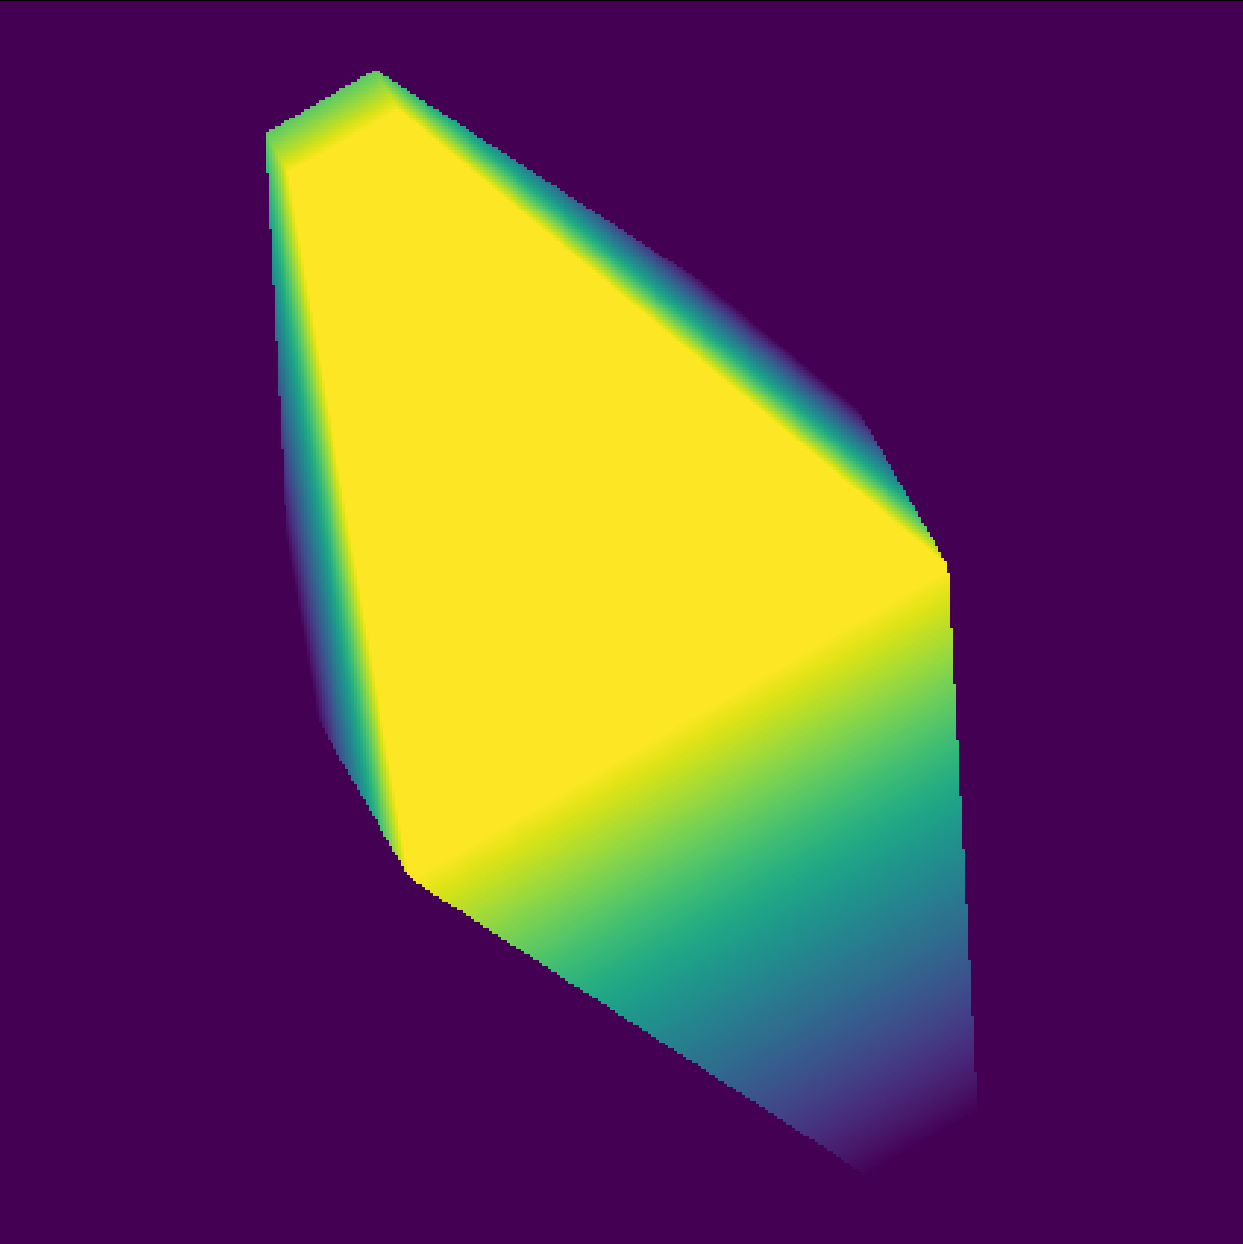
\includegraphics[width=.95\textwidth]{./immagini/bipiramid_singola.png}
        \caption{}
        \label{fig:bipiramid1}
    \end{subfigure}
    \hfill
    \begin{subfigure}[b]{0.3\textwidth}
        % bipiramid_doppia
        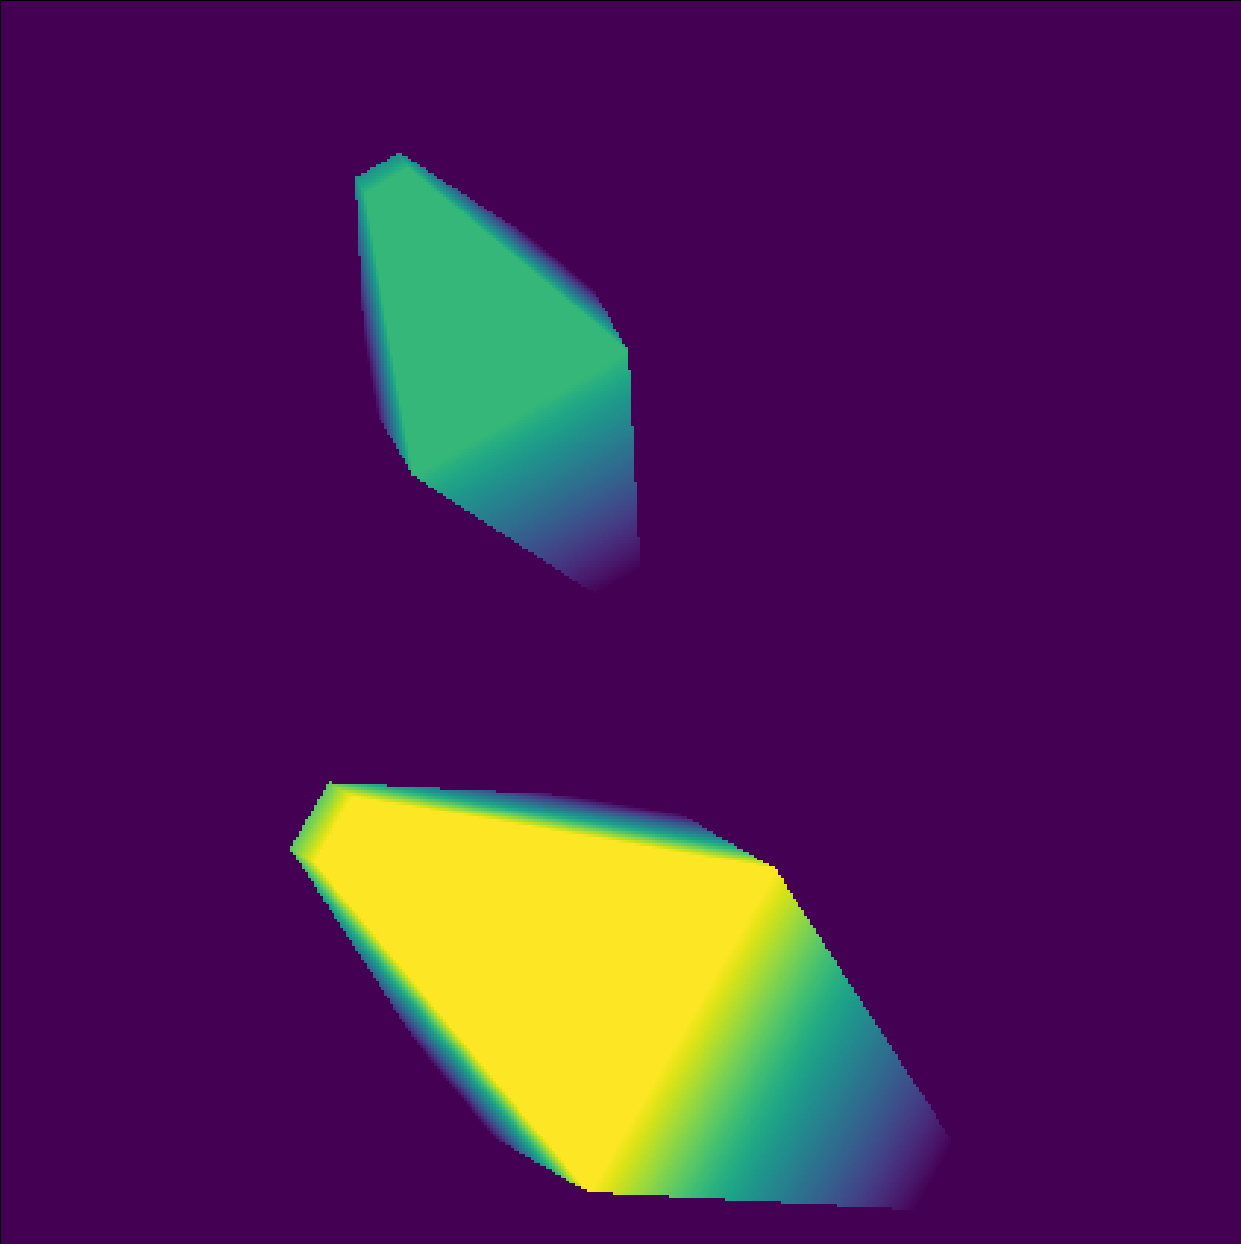
\includegraphics[width=.95\textwidth]{./immagini/bipiramid_doppia.png}
        \caption{}
        \label{fig:bipiramid2}
    \end{subfigure}
    \hfill
    \begin{subfigure}[b]{0.3\textwidth}
        % bipiramid_statistica
        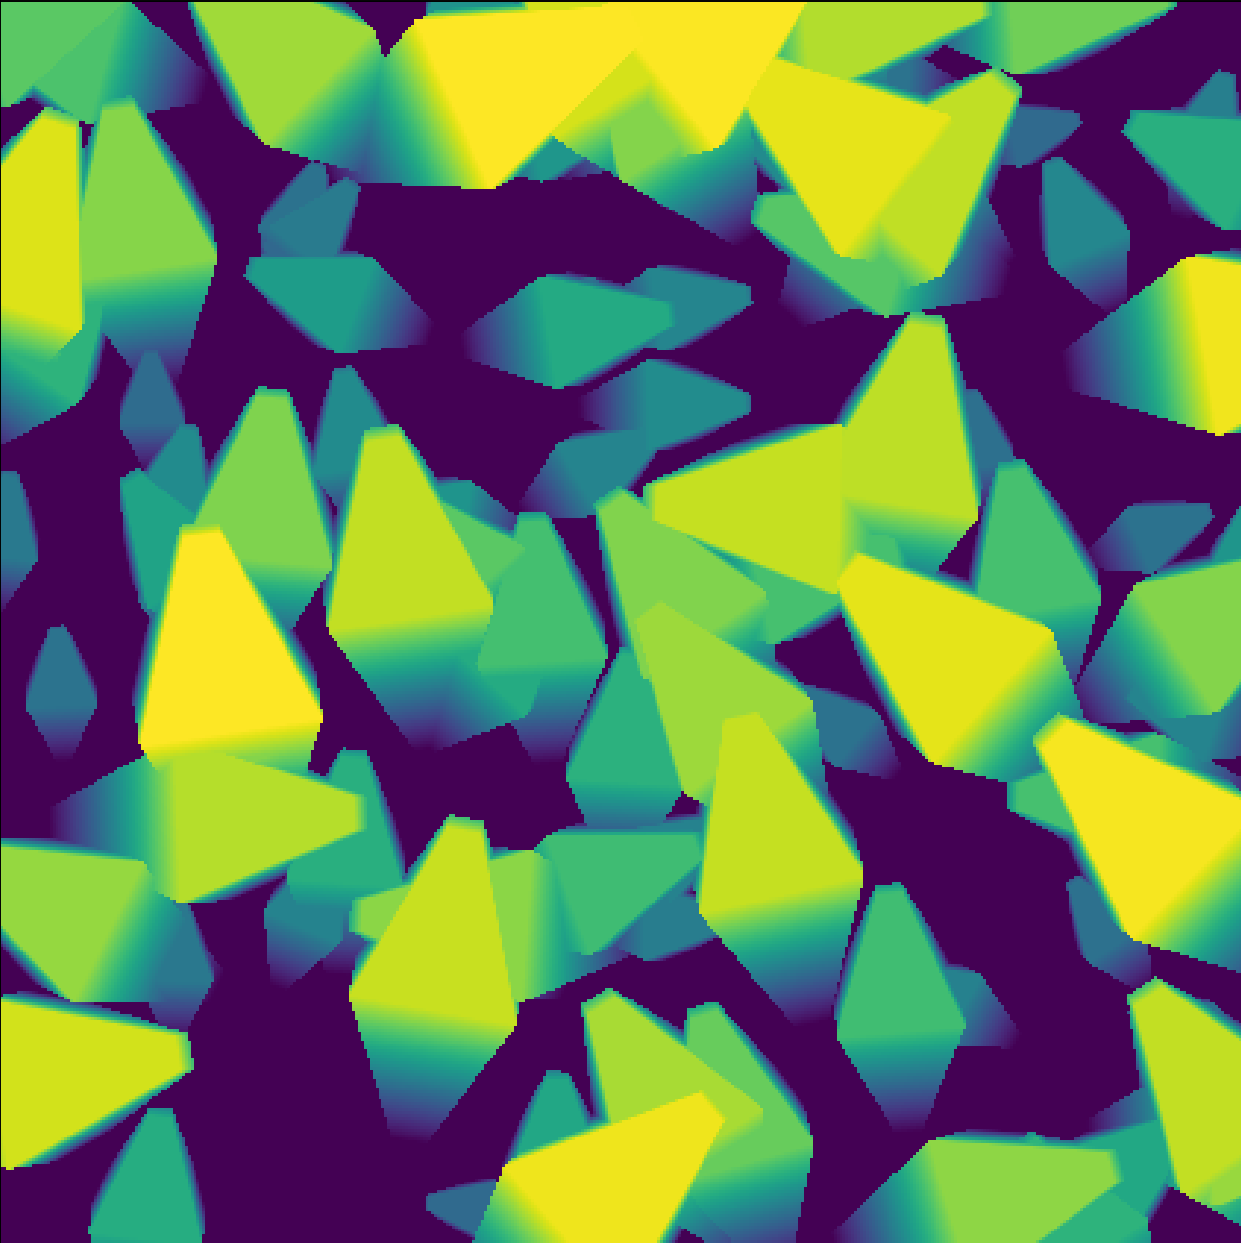
\includegraphics[width=.95\textwidth]{./immagini/bipiramid_statistica.png}
        \caption{}
        \label{fig:bipiramid3}
    \end{subfigure}
    \caption{Example of usage of bipiramids: a) Single b) Double c) Statistic}
    \label{fig:bipiramid_type}
\end{figure}